\section{目的與規格對照}
依 Lab 10（PDF 第 39--43 頁）完成四項要求。第一個 netlist 掃描反相器尺寸 1--4 倍及負載 0/0.1/0.2/0.3 pF，固定輸入邊緣參數 0.2 ns，同時涵蓋固定負載改尺寸、固定尺寸改負載、尺寸與負載共同掃描三步。第二個 netlist 固定尺寸 1 倍，掃描輸入邊緣 0.2/0.4/0.6/0.8 ns 及上述四種負載，對應表 10.1。總計兩個 netlist、32 個變體全部完成求解及量測。

\section{電路與延遲模型}
單位反相器採 $W_p/W_n=1.8/0.6\,\mu$m、$L=0.25\,\mu$m，尺寸倍數同時乘到兩種寬度。輸出接理想負載電容；標示零負載時只加入 $10^{-21}$ F 的數值極小量，模型自身寄生效應仍保留。

以 $z=(t_{pHL}+t_{pLH})/2$ 為平均延遲，先在固定輸入邊緣下擬合 $z=A_0+A_1C_L$。再以負載 $x$（pF）、PULSE 邊緣參數 $y$（ns）建立講義的雙線性形式
\[z=A+Bx+Cy+Dxy.\]
這是有限工作區間的近似，不是晶體管方程的精確解；全部原始 $t_{pHL}$、$t_{pLH}$、輸出上升及下降時間都保留在 CSV。

\section{模擬設定與量測定義}
本次使用獨立提供的 MOS 模型，電源為 1.0 V、溫度為 $27\,^{\circ}$C，並保留講義的電路拓樸及下列比較條件。1 V 是本次模擬設定，並非由公開模型文件確認的元件額定值；不能把講義舊製程的數值當成此次模型的驗收值。

模擬使用 HSPICE S-2021.09、RUNLVL=6。表格取自實際原生量測結果，圖形由實際列印數據重繪；每個變體都完整重設掃描參數及溫度，避免前一個變體的設定殘留。數值求解完成與量測成功，不等於已驗證製程可靠度。加密模型區塊的內部警告仍無法完整檢視。
PULSE 的 SLEW 參數是從 0 到 100\% 的線性斜坡時間，其 10--90\% 區間為 $0.8\times$SLEW。這與輸出採 10--90\% 量測的定義不同，報告明確區分。週期為 25 ns，輸入初始延遲 2 ns、脈寬 10 ns；暫態 50 ns、列印間距 5 ps。傳播延遲採輸入／輸出 50\% 交越。

\section{固定輸入邊緣的線性擬合}
下表以 ns、pF 為單位，殘差為四個負載點的最大絕對誤差。

\begin{center}\small
\begin{tabular}{llll}
\toprule
尺寸 & $A_0$ (ns) & $A_1$ (ns/pF) & Max residual (ps) \\
\midrule
1 & 0.05936 & 3.69754 & 8.96 \\
2 & 0.05939 & 1.87448 & 8.77 \\
3 & 0.05880 & 1.26966 & 7.53 \\
4 & 0.05875 & 0.96623 & 7.18 \\
\bottomrule
\end{tabular}
\end{center}
\begin{figure}[htbp]
\centering
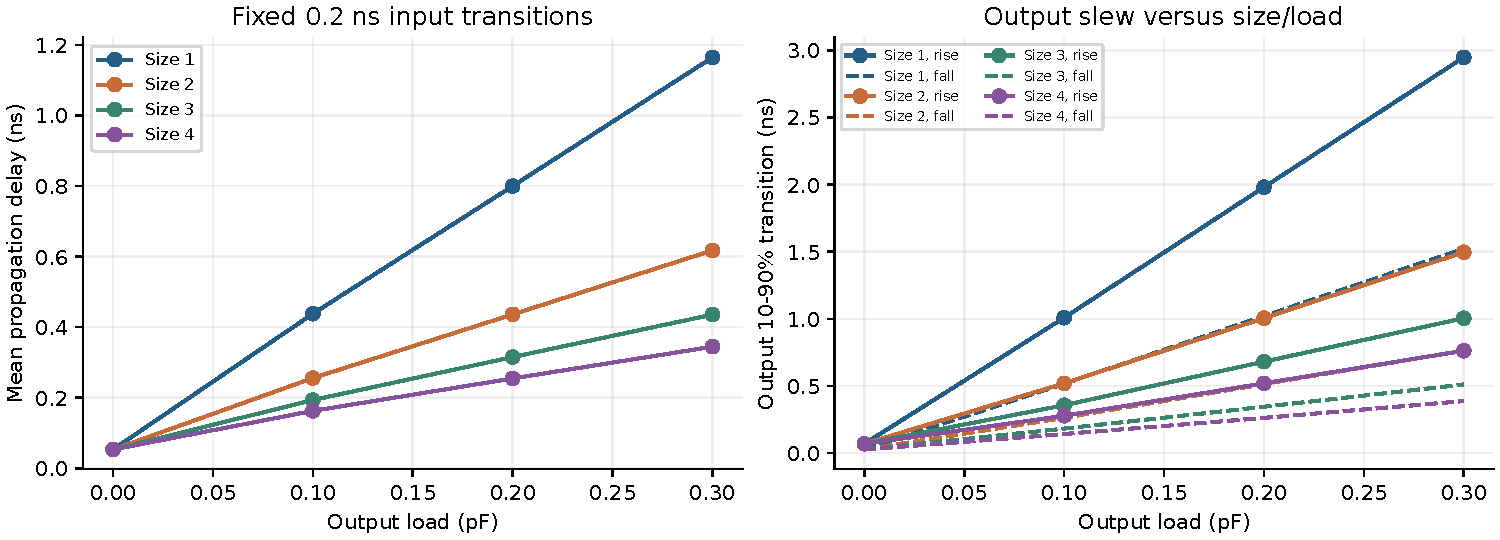
\includegraphics[width=\linewidth]{figures/linear_delay.pdf}
\caption{固定邊緣下的負載延遲，以及輸出上升／下降時間。}
\end{figure}
\section{負載與輸入邊緣的二維結果}
下表為平均傳播延遲（ns），行為輸入斜坡參數、列為輸出負載。

\begin{center}\small
\begin{tabular}{lllll}
\toprule
Ramp (ns) & 0 pF & 0.1 pF & 0.2 pF & 0.3 pF \\
\midrule
0.2 & 0.0530 & 0.4381 & 0.8000 & 1.1649 \\
0.4 & 0.0668 & 0.4843 & 0.8484 & 1.2132 \\
0.6 & 0.0768 & 0.5326 & 0.8973 & 1.2600 \\
0.8 & 0.0850 & 0.5808 & 0.9472 & 1.3067 \\
\bottomrule
\end{tabular}
\end{center}
\[z=0.038107+3.583427x+0.109639y+0.556701xy\quad\text{(ns)}.\]
使用同一組 16 點資料時，只考慮負載的模型 RMSE 為 51.17 ps；加入斜坡及交互項後降至 23.64 ps，最大殘差仍有 52.14 ps。這是資料內擬合誤差，並非獨立驗證集的預測誤差。
\begin{figure}[htbp]
\centering
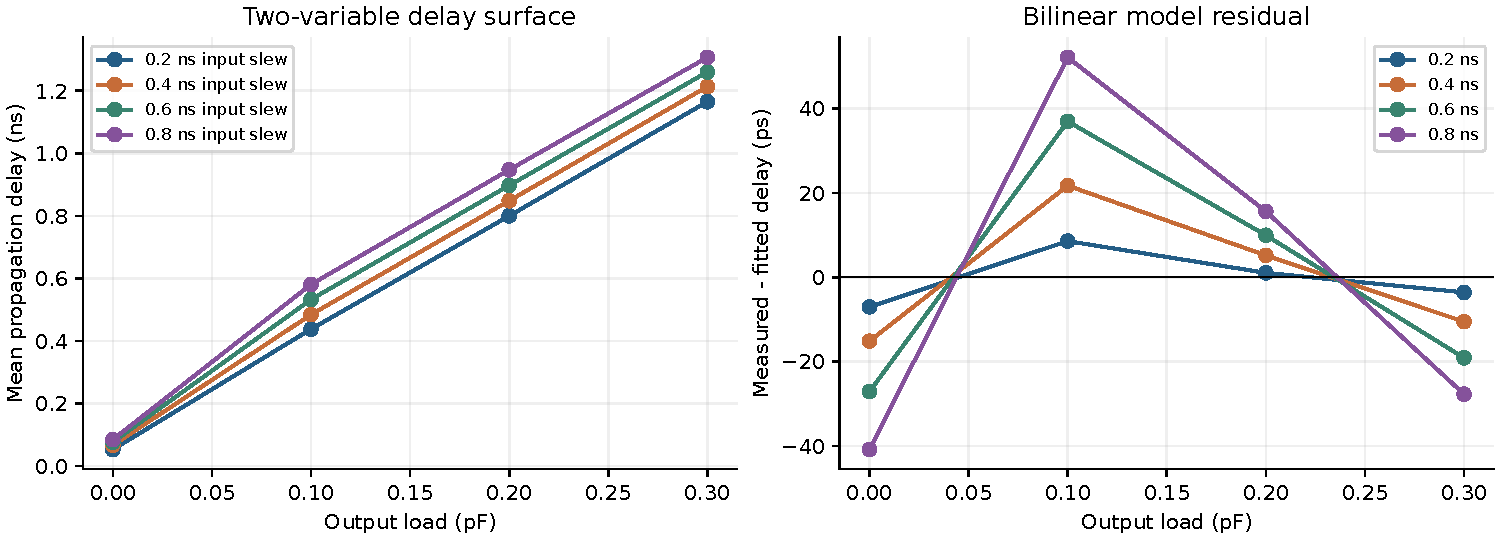
\includegraphics[width=\linewidth]{figures/nonlinear_delay.pdf}
\caption{輸入斜坡改變延遲曲面，雙線性近似仍有可見殘差。}
\end{figure}
\section{討論}
提高尺寸降低每單位負載的延遲斜率；本次從尺寸 1 的 3.6975 ns/pF 降至尺寸 4 的 0.9662 ns/pF。非零截距反映內部寄生、有限輸入斜坡與模型擬合效應，不能直接解讀成單一固定的物理電容。

固定負載時，慢輸入使平均傳播延遲增加，因此忽略輸入邊緣會產生系統性誤差。雙線性模型改善平均誤差，但在低負載及慢斜坡附近仍有曲率，適合改用更細的查表資料與插值。圖中的不同線條相連僅便於觀察，不表示已驗證範圍外的線性外插。

\section{可重現檔案}
本實驗上傳下列 netlist；模型設定以註解標記保留，模型檔與其路徑均不隨報告上傳。執行前須在本機補入合法可用的模型設定。
\begin{itemize}
\item \texttt{01\_size\_load.sp}
\item \texttt{02\_slew\_load.sp}
\end{itemize}
每一個變體的完整量測值位於本 lab 的 \texttt{results}，並附代表性波形 CSV、分析結果與規格對照清單。波形 CSV 最多保留 2501 個均勻取樣點；直接量測未降採樣。完整原始 listing 留在本機。

